%!TEX root = ../tesis.tex
\section{Modelos Ocultos de Markov}
\label{sec:hmm}

Para introducir el concepto de modelo oculto de Markov (\gls{hmm} por sus siglas en ingl\'es), 
en el cual se basa el proceso de reconocimiento del habla que se busca explicar, 
se utilizar\'a un ejemplo cl\'asico de la literatura relacionada con el tema.
El ejemplo se denomina \emph{El modelo de la urna y la pelota} \cite{Rabiner89atutorial}:

\begin{figure}[H] 
\centering
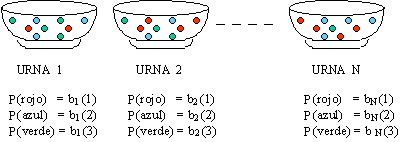
\includegraphics[width=0.8\textwidth]{./graphics/urnas.png}
\caption{Representaci\'on gr\'afica del modelo de la urna y la pelota \cite{LleidaModelado}.}
\label{figure:urnas}
\end{figure}

\begin{quote}
	Se asume que hay N urnas (grandes) de vidrio en una habitaci\'on. Dentro de cada urna hay un gran 
	n\'umero de pelotas de colores.
	Un genio est\'a en la habitaci\'on y, de acuerdo a un proceso aleatorio, elige una urna inicial. 
	De esta urna extrae una pelota de manera aleatoria y su color se anota como la observaci\'on, 
	pues el observador desconoce la urna de donde sali\'o la pelota.
	La pelota se coloca de nuevo en la urna y se repiten la selecci\'on de la urna y la pelota respectivamente.
	Este proceso genera una secuencia aleatoria de colores.
\end{quote}

En el caso mencionado, puden distinguirse dos procesos estoc\'asticos:
\begin{itemize}
	\item Del primer proceso se obtiene como salida una secuencia de urnas. Sin embargo, el observador
	no puede visualizar esta secuencia, es decir, la misma permanece oculta.
	\item Del segundo proceso se obtiene como salida una secuencia de colores. La probabilidad de observar
	un color depende de la urna seleccionada previamente, debido a que la cantidad de pelotas de un determinado
	color var{\'\i}a en cada urna.
\end{itemize}

Este sencillo sistema puede modelarse como un modelo oculto de Markov definiendo los siguientes par\'ametros:
\begin{enumerate}
	\item El n\'umero de urnas, a las cuales se denomina estados del modelo.
	\item La cantidad de colores posibles de las pelotas en las urnas, a los cuales se 
	denomina s{\'\i}mbolos observables.
	\item Una funci\'on que determina la transici\'on entre urnas.
	\item Una funci\'on que determina la elecci\'on de una pelota de determinado color, dada una urna.
	\item Una funci\'on que determina la elecci\'on de la urna inicial.
\end{enumerate}

Con la ayuda de este ejemplo, podemos definir formalmente un \gls{hmm}. Un modelo oculto de Markov es un 
aut\'omata finito estoc\'astico entrenable \cite{KouemouHistory2011}, que implica un doble proceso estoc\'astico:

\begin{itemize}
\item El primer proceso, que produce una secuencia de estados, no es observable. Esto es, la secuencia de estados 
que produce permanece oculta.
\item El segundo proceso produce una secuencia de observaciones, donde la probabilidad de 
una observaci\'on est\'a dada por una funci\'on definida para cada estado correspondiente al primer proceso.
\end{itemize}

Un modelo oculto de Markov puede ser caracterizado mediante los siguientes elementos \cite{Rabiner89atutorial}:

\begin{enumerate}
	\item $N$, el n\'umero de estados del modelo. Se representan los estados individuales como: 
		\begin{align}
			S=\{S_1,S_2,\ldots,S_N\}\label{eq:hmmS}
	\end{align}

	\item $M$, el n\'umero de s{\'\i}mbolos observables por estado. Se representan los s{\'\i}mbolos individuales 
		como: 
		\begin{align}
			V=\{v_1,v_2,\ldots,v_M\}\label{eq:hmmV}
	\end{align}

	\item La distribuci\'on de probabilidad de transici\'on de estados $A = \left\{a_{ij}\right\}$.
		Siendo $q_t$ el estado del modelo generado en el tiempo $t$, puede definirse $a_{ij}$ como:

		\begin{align}
			a_{ij} = P[q_{t+1} = S_j \mid q_t = S_i], & & 1 \leq i,j & \leq N\label{eq:hmmA}
		\end{align}

	\item La distribuci\'on de probabilidad de los s{\'\i}mbolos observables en el estado $j$, $b_j(v_k)$. 
		Esta distribuci\'on es una funci\'on de la observaci\'on $v_k$, definida en cada estado.
		Siendo $q_t$ el estado del modelo generado en el tiempo $t$:

		\begin{align}
			b_j(v_k) = P[v_k \text{ en el momento } t \mid q_t = S_j], & & 1 \leq j & \leq N \label{eq:hmmB}
			\\& & 1 \leq k & \leq M \nonumber
		\end{align}

	\item La distribuci\'on de probabilidad del estado inicial $\pi=\left\{\pi_i\right\}$, donde:
		\begin{align}
			\pi_i = P[q_1=S_i], & & 1 \leq i \leq N \label{eq:hmmPI}
		\end{align}
\end{enumerate}

\begin{figure}[H] 
\centering
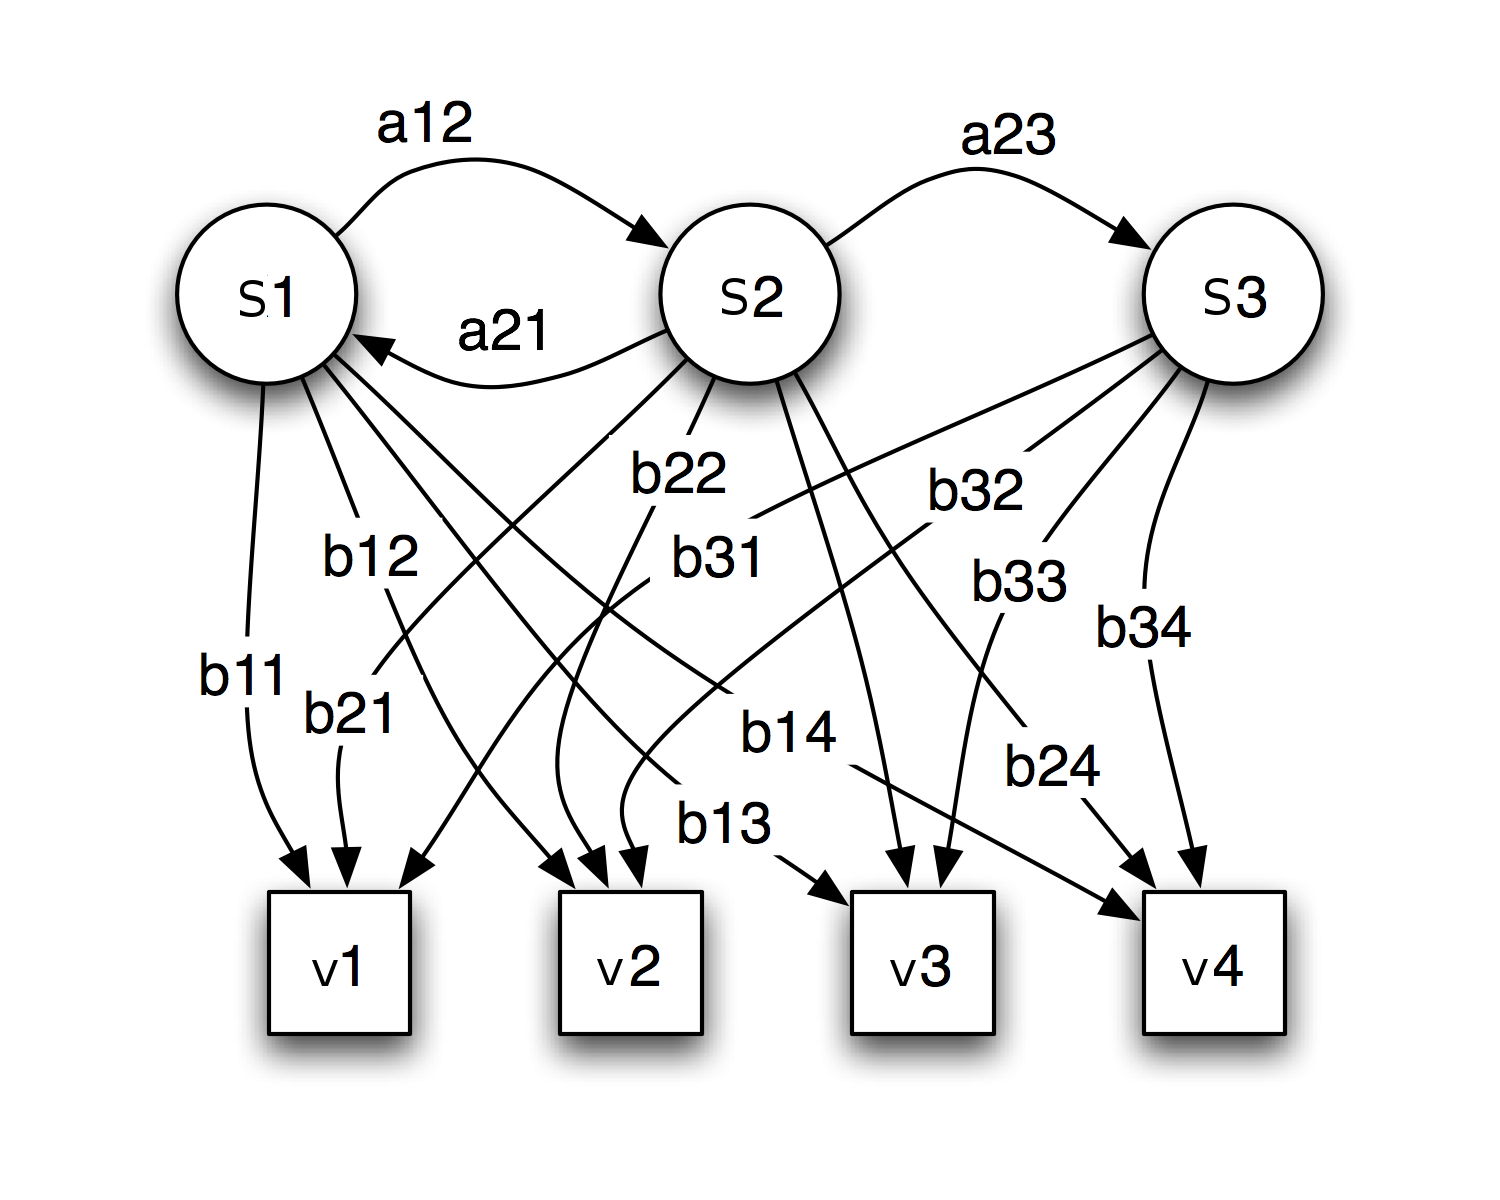
\includegraphics[width=0.8\textwidth]{./graphics/hmm.png}
\caption{Representaci\'on gr\'afica de un modelo oculto de Markov.}
\label{figure:hmm}
\end{figure}